\documentclass[tikz,border=2pt]{standalone}
\usepackage{amsmath,amssymb}
\usepackage{tikz}
\usetikzlibrary{arrows.meta}

\begin{document}
% Shortest path as a binary program: x_ij = 1 on the selected directed edges; one unit of
% flow leaves the origin and enters the destination, and flow is conserved elsewhere.
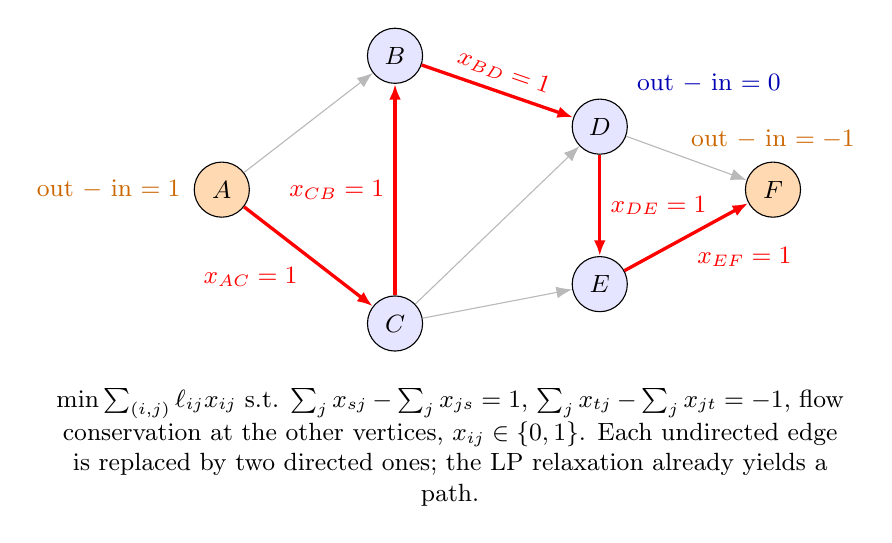
\begin{tikzpicture}[every node/.style={font=\small}, >={Latex[length=2mm]}, v/.style={draw, circle, fill=blue!10, minimum size=7mm, inner sep=0pt}]
	\node[v, fill=orange!30] (A) at (0,0) {$A$};
	\node[v] (B) at (2.2,1.7) {$B$};
	\node[v] (C) at (2.2,-1.7) {$C$};
	\node[v] (D) at (4.8,0.8) {$D$};
	\node[v] (E) at (4.8,-1.2) {$E$};
	\node[v, fill=orange!30] (F) at (7.0,0) {$F$};
	\foreach \a/\b in {A/B, C/D, C/E, D/F} {\draw[gray!55, ->] (\a) -- (\b);}
	\draw[red, very thick, ->] (A) -- (C) node[midway, below left] {$x_{AC}=1$};
	\draw[red, very thick, ->] (C) -- (B) node[midway, left] {$x_{CB}=1$};
	\draw[red, very thick, ->] (B) -- (D) node[midway, above, sloped] {$x_{BD}=1$};
	\draw[red, very thick, ->] (D) -- (E) node[midway, right] {$x_{DE}=1$};
	\draw[red, very thick, ->] (E) -- (F) node[midway, below right] {$x_{EF}=1$};
	\node[orange!80!black, anchor=east] at (-0.4,0) {out $-$ in $=1$};
	\node[orange!80!black, anchor=south] at (7.0,0.4) {out $-$ in $=-1$};
	\node[blue!70!black, anchor=south west] at (5.15,1.1) {out $-$ in $=0$};
	\node[anchor=north, align=flush center, text width=10cm] at (2.9,-2.4) {$\min\sum_{(i,j)}\ell_{ij}x_{ij}$ s.t. $\sum_jx_{sj}-\sum_jx_{js}=1$, $\sum_jx_{tj}-\sum_jx_{jt}=-1$, flow conservation at the other vertices, $x_{ij}\in\{0,1\}$. Each undirected edge is replaced by two directed ones; the LP relaxation already yields a path.};
\end{tikzpicture}
\end{document}
